\section{Proofs}
\label[appendix]{app:proofs}

\subsection{Second moments under He initialisation}

We prove \cref{cor:he}.
Put $h^0=x$ and $h^k=\relu(W^kh^{k-1})$. Given $h^{k-1}$, the coordinates of
$W^kh^{k-1}$ are $N(0,s_k^2\|h^{k-1}\|^2)$, where $s_k^2$ is the weight variance
of layer $k$. For a centred Gaussian $z$, symmetry gives
$\E\,\relu(z)^2=\tfrac12\E z^2$. Hence
$\E\bigl[\|h^k\|^2\mid h^{k-1}\bigr]=\tfrac12n_ks_k^2\|h^{k-1}\|^2$. With
$s_k^2=2/n_{k-1}$ this reads $\E\|h^k\|^2/n_k=\E\|h^{k-1}\|^2/n_{k-1}$, so
$\E\|h^L\|^2/n_L=\|x\|^2/d$. Given $h^L$, the output is
$N(0,(2/n_L)\|h^L\|^2)$, so $\E f_\theta(x)=0$ and
$\E f_\theta(x)^2=2\,\E\|h^L\|^2/n_L=2\|x\|^2/d$. The third identity follows by
expanding the square. With $s_k^2=1$ the recursion is
$\E\|h^k\|^2=\tfrac12n_k\E\|h^{k-1}\|^2$ and $\E f_\theta(x)^2=\E\|h^L\|^2$. \qed

\subsection{Area of a tube around a curve}

We prove \cref{lem:tube-area}.

\emph{Polygonal paths.} Let $Q$ be a polygonal path with vertices
$q_0,\dots,q_k$ and segments of lengths $s_1,\dots,s_k$. For a segment $[a,b]$,
the tube $N_r([a,b])$ is a rectangle of sides $|b-a|$ and $2r$ with a half-disc
of radius $r$ at each end. Its area is $2r|b-a|+\pi r^2$, and it contains the
closed disc $\bar B_r(a)$, so $N_r([a,b])\setminus\bar B_r(a)$ has area
$2r|b-a|$. Let $Q_j$ be the path up to $q_j$. Then $N_r(Q_0)=\bar B_r(q_0)$ has
area $\pi r^2$, and $N_r(Q_j)=N_r(Q_{j-1})\cup N_r([q_{j-1},q_j])$. Since
$\bar B_r(q_{j-1})\subset N_r(Q_{j-1})$, passing from $Q_{j-1}$ to $Q_j$ adds at
most the area of $N_r([q_{j-1},q_j])\setminus\bar B_r(q_{j-1})$, which is
$2rs_j$. By induction the area of $N_r(Q)$ is at most $\pi r^2+2r\sum_js_j$.

\emph{Rectifiable curves.} Let $\gamma:[0,1]\to\R^2$ be continuous with length
$l<\infty$ and image $S$. Fix $\varepsilon>0$. By uniform continuity there is a
partition $0=t_0<\dots<t_k=1$ such that each arc $\gamma([t_{j-1},t_j])$ has
diameter at most $\varepsilon$. Let $Q$ be the polygonal path through the
points $\gamma(t_j)$; its length is at most $l$ by the definition of length.
Every point of $S$ is within $\varepsilon$ of a vertex of $Q$, and $S$ is
compact, so $N_r(S)\subset N_{r+\varepsilon}(Q)$. By the first step the area of
$N_r(S)$ is at most $2l(r+\varepsilon)+\pi(r+\varepsilon)^2$. Let
$\varepsilon\to0$. \qed

\subsection{Arc length of the sine}

For $f(x)=\sin(w\pi x+\varphi)$ on $[-1,1]$ the arc length is
$l(w)=\int_{-1}^{1}\sqrt{1+w^2\pi^2\cos^2(w\pi x+\varphi)}\,dx$. Since
$c\le\sqrt{1+c^2}\le1+c$ for $c\ge0$,
\[
  I\le l(w)\le2+I,\qquad
  I=w\pi\int_{-1}^{1}|\cos(w\pi x+\varphi)|\,dx=\int_{\varphi-w\pi}^{\varphi+w\pi}|\cos u|\,du .
\]
The function $|\cos|$ has period $\pi$ and integral $2$ over a period. An
interval of length $2\pi w$ contains $\lfloor2w\rfloor$ full periods and a
remainder shorter than one period, so $4w-2\le I\le4w+2$. Hence
$4w-2\le l(w)\le4w+4$ and $l(w)/w\to4$. With peak $p$ the same argument gives
$l(w)/w\to4p$, in agreement with \cref{tab:freq} ($4\times0.816\times64=208.9$).

\subsection{The constant for the sine}

We derive the second limit of \cref{prop:sine}.

Take $p=1$ and fix a phase $\varphi$ and a height $y_0\in(-1,1)$. Put
$a=\arcsin(y_0)\in(-\pi/2,\pi/2)$.

\emph{Crossings.} The curve is at height $y_0$ where $w\pi x+\varphi$ equals
$a$ or $\pi-a$ modulo $2\pi$. These are two lattices in $x$, each of period
$2/w$, and consecutive crossings are separated alternately by
\[
  g_1=\frac1w\Bigl(1-\frac{2a}{\pi}\Bigr),\qquad
  g_2=\frac1w\Bigl(1+\frac{2a}{\pi}\Bigr),\qquad g_1+g_2=\frac2w .
\]

\emph{Horizontal distance.} Let $h(x_0,y_0)$ be the distance from $x_0$ to the
nearest crossing at height $y_0$. A point $x_0$ falls in a gap of length $g$
with probability proportional to $g$, and its mean distance to the nearer end
is then $g/4$. Averaging over $x_0$ across whole periods,
\[
  \frac{g_1^2+g_2^2}{4(g_1+g_2)}=\frac{1}{4w}\Bigl(1+\frac{4a^2}{\pi^2}\Bigr).
\]
The interval $[-1,1]$ contains whole periods and end pieces of total length at
most $4/w$, on which $h\le2/w$ for $w\ge1$. So the mean of $h$ over $x_0$
uniform on $[-1,1]$ differs from the display by $O(1/w^2)$.

\emph{Average over heights.} For $y_0$ uniform on $[-1,1]$, with $y=\sin t$,
\[
  \E\,\arcsin(y_0)^2=\int_0^1\arcsin(y)^2\,dy=\int_0^{\pi/2}t^2\cos t\,dt
  =\Bigl[t^2\sin t+2t\cos t-2\sin t\Bigr]_0^{\pi/2}=\frac{\pi^2}{4}-2 .
\]
Therefore
$w\,\E h\to\frac14\bigl(1+\frac{4}{\pi^2}(\frac{\pi^2}{4}-2)\bigr)=\frac14\bigl(2-\frac{8}{\pi^2}\bigr)$.

\emph{From horizontal to Euclidean distance (outline).} It remains to show that
$w\,\E\,\nd$ and $w\,\E h$ have the same limit. Clearly $\nd\le h$. For the
other direction fix $\eta\in(0,1)$ and suppose $|y_0|\le1-\eta$. Each monotone
stroke of the curve is the graph of $x$ as a function of the height $y$, with
derivative $1/(w\pi\sqrt{1-y^2})$. On the window of heights within $2/w$ of
$y_0$ this derivative is at most
$\kappa=1/\bigl(w\pi\sqrt{1-(1-\eta+2/w)^2}\bigr)$ once $2/w<\eta$, and
$\kappa\to0$ as $w\to\infty$. Points of the curve outside the window are
further than $2/w\ge h$ from $(x_0,y_0)$. Inside the window,
\cref{thm:sandwich} applies to each stroke with the roles of $x$ and $y$
exchanged, and gives $\nd\ge h/\sqrt{1+\kappa^2}$. The points with
$|y_0|>1-\eta$ have probability $\eta$ and $\nd\le h\le2/w$, so they change
$w\,\E\,\nd$ and $w\,\E h$ by at most $2\eta$ each. Letting $w\to\infty$ and
then $\eta\to0$ gives the claim. We have not written out the measurability and
edge details of this last step, and for that reason label the result as
leading-order; the numerical check is in \cref{sec:saturation}.

\subsection{The band-edge floor}

We prove \cref{prop:floor}.

\emph{Lower bound.} The curve lies in the band $|y|\le p$. A point $(x_0,y_0)$
is therefore at distance at least $\max(0,|y_0|-p)$ from it. For $y_0$ uniform
on $[-1,1]$, $\E\max(0,|y_0|-p)=\int_p^1(t-p)\,dt=(1-p)^2/2$.

\emph{Upper bound.} We use the following fact: if $\Lambda\subset\R$ is a
lattice of period $2/w$ with $w\ge1$, every $x_0\in[-1,1]$ has a point of
$\Lambda\cap[-1,1]$ within $2/w$. Indeed, let $x_L\le x_0<x_R=x_L+2/w$ be the
neighbours of $x_0$ in $\Lambda$. If $x_L\ge-1$ take $x_L$. Otherwise
$x_R<-1+2/w\le1$ and $x_R>x_0\ge-1$, so take $x_R$.

If $|y_0|\le p$, the crossings of the curve at height $y_0$ contain a lattice
of period $2/w$, so there is a point of the curve at height $y_0$ within $2/w$
of $x_0$, and the distance is at most $2/w$. If $y_0>p$, the maxima of the
curve form a lattice of period $2/w$ at height $p$, so the distance is at most
$\sqrt{(y_0-p)^2+(2/w)^2}\le(y_0-p)+2/w$. The case $y_0<-p$ is the same with
the minima. In every case the distance is at most $\max(0,|y_0|-p)+2/w$, for
every phase. Taking expectations gives the upper bound. \qed

\section{ReLU chains and polarizers}
\label[appendix]{app:chains}

The statements in this appendix are proved in Lean. The main results do not use
them. They concern claim (P) for the simplest ReLU networks, and an analogy
with polarizers that explains why a turn needs more than one neuron.

\paragraph{One neuron per layer.} The network
$\relu\bigl(w_1\relu(w_2\cdots\relu(w_Lx+b_L)\cdots)+b_1\bigr)$ is monotone, for
every depth and all weights and biases: each layer is a non-decreasing or
non-increasing function of its input, and a composition of such functions is
again one. Such a network never turns.

\paragraph{Two neurons per layer.} Let $T(x)=2\relu(x)-4\relu(x-\tfrac12)$, one
layer with two neurons, which folds $[0,1]$ in half. For every $L$ and every
integer $0\le k\le2^L$, the $L$-fold composition satisfies $T^L(k/2^L)=0$ if
$k$ is even and $1$ if $k$ is odd. So $L$ layers of two neurons draw a curve
that turns $2^L-1$ times. Moreover, for $x\in[0,1]$,
\[
  \sin^2\!\bigl(\tfrac{\pi}{2}\,T^L(x)\bigr)=\sin^2\!\bigl(2^{L}\cdot\tfrac{\pi}{2}\,x\bigr),
\]
so that, seen through the fixed function $\sin^2(\tfrac\pi2\,\cdot)$, $L$ folds
are a single Fourier mode of frequency $2^L$. Depth in such a network plays
the role of the logarithm of frequency in \cref{sec:fourier}.

\paragraph{ReLU as a projection.} In the plane, the coordinatewise ReLU sends a
point to the nearest point of the positive quadrant. Let $R_\theta$ be the
rotation by $\theta$ and $r\ge0$. A layer that rotates and then applies the
ReLU acts on a point on the edge of the quadrant by
\[
  \relu\bigl(R_{-\theta}(r,0)\bigr)=
  \begin{cases}(r\cos\theta,\,0)&0\le\theta\le\pi/2,\\(0,0)&\pi/2\le\theta\le\pi,\end{cases}
\]
so $N$ such layers with $\theta\le\pi/2$ keep the length $r\cos^N\theta$.

\paragraph{Polarizers.} A linear polarizer with axis at angle $\phi$ is the
orthogonal projection $P_\phi$ onto that direction. Writing $u_\psi$ for the
unit vector at angle $\psi$, we have $P_\phi(a\,u_\psi)=a\cos(\phi-\psi)\,u_\phi$
(Malus's law for the amplitude). After $k$ plates at angles
$\theta,2\theta,\dots,k\theta$ the vector $a\,u_0$ has become
$a\cos^k\theta\;u_{k\theta}$. A single plate at $90^\circ$ delivers nothing, a
plate at $45^\circ$ followed by one at $90^\circ$ delivers half the length, and
a quarter turn made in $N\ge2$ equal steps delivers
$\cos^N(\pi/2N)\ge1-\pi^2/(8N)$. A turn made in many small steps loses little,
and a turn made in one step loses everything. The rotate-then-ReLU layer above
obeys the same rule, and a network with one neuron per layer has no
intermediate direction to turn through. The comparison stops there: a stack of
projections onto lines is a linear map, and a stack of ReLU layers is not.

\paragraph{Chains without memory.} For any stack of maps applied in turn, two
inputs that reach the same state stay together, the number of distinct states
of a finite set of inputs never increases, and a state that every layer fixes
is never left.

\section{What went wrong in the first version}
\label[appendix]{app:wrong}

The first scripts, written in August 2025, appeared to support the conjecture,
and a draft paper reported that support. Three of their measurements were not
what they were described as. The repository keeps the scripts unchanged, with a
warning, and a script that reproduces each defect.

\begin{enumerate}\setlength{\itemsep}{1pt}
\item \emph{The ``distance'' was a neuron count.} The core metric compared the
label with the number of active neurons of the network, which is about half the
width. It measured $4.9$ at width 10 and $80.1$ at width 160. It grows linearly
with width, the opposite of the conjecture, and was captioned as support for
it. Its apparent independence of the input dimension was the absence of any
dependence on the data.
\item \emph{The scaling law was the output fading.} A power law with exponent
about $0.42$ was reported for $\|\mathrm{net}(x)-x\|$, the distance from the
output of a network to its own input, on a $2\to w\to w\to2$ ReLU stack with
Xavier initialisation \citep{glorot2010understanding}. In that setup the output
shrinks towards zero as the width grows, so the metric converges to $\|x\|$, the
score of a network that returns nothing: $1.3186$ at width 2 and $1.2325$ at
width 128, against $1.2299$ for the zero function.
\item \emph{The one-dimensional case measured against a diagonal.} One
coordinate of each random point was used as both $x$ and $y$, which placed
every point on the line $y=x$.
\end{enumerate}

The original derivation also estimated the mean distance as a power of the
uncovered fraction of the region and drew a conclusion about diminishing returns
that the formula does not support; \cref{thm:tube} replaces that estimate.

Two later corrections were numerical and concern the experiments reported here.

\begin{enumerate}\setlength{\itemsep}{1pt}
\item \emph{Fixed sampling grid (corrected 19 September 2026).} Curves were
first sampled on a fixed grid of 4000 points. At $w=64$ the steepest slope of
the sine is about $164$, so consecutive samples were about $0.08$ apart
vertically, more than the distances being measured. The nearest-point distance
was overestimated from $w\approx32$ upwards ($0.0279$ reported at $w=64$,
against $0.0207$), which produced a spurious plateau. The grid is now sized for
each frequency.
\item \emph{Wrong stroke (corrected 11 November 2026).} The replacement refined
the distance only on the two segments next to the nearest sample. Once the gap
$1/w$ between neighbouring strokes is below the sample spacing $0.002$, the
nearest sample can lie on the wrong stroke. In the control of
\cref{sec:saturation} this overestimated the mean distance by $11\%$ at
$w=1000$ ($0.000324$ against $0.000292$). The routine now projects onto every
segment that can contain the nearest point, is exact for the polyline, and
agrees with a brute-force reference to better than $10^{-6}$ from $w=0.25$ to
$w=1000$ at both amplitudes. \Cref{tab:freq,tab:line} did not change in the
digits shown. The tail fits of \cref{sec:saturation} moved slightly: before the
correction they read $\beta=0.978$, $c=0.236$, a predicted knee of $55.7$, and
$0.285\,w^{-0.989}$ for the control.
\end{enumerate}

\section{Experimental details}
\label[appendix]{app:details}

All scripts are in the \texttt{scripts/} folder of the repository and use fixed
random seeds.

\begin{itemize}\setlength{\itemsep}{1pt}
\item \texttt{frequency\_isolation.py}: \cref{tab:freq,tab:line}. 3000 trials of
30 points; 100 stratified phases per frequency; about ten seconds.
\item \texttt{saturation\_scaling.py}: \cref{tab:knee} and the fits of
\cref{sec:saturation}. $30\,000$ points per $n$, 16 phases per frequency, 25
frequencies logarithmically spaced in $[1,1000]$, 300 bootstrap resamples; the
control uses $n=100$. Several minutes.
\item \texttt{initial\_mse.py}: \cref{tab:mse}.
\item \texttt{random\_relu\_length.py}: \cref{tab:relu-full}.
\item \texttt{fourier\_params.py}: \cref{tab:fourier}. 20 data sets and 20
random starts for each number of terms; the number of gradient steps is
computed exactly in the eigenbasis of the kernel.
\item \texttt{curves.py}: the sine geometry and the exact point-to-polyline
distance shared by the first two scripts.
\item \texttt{audit\_legacy\_metrics.py}: reproduces the three defects of
\cref{app:wrong}.
\item \texttt{readme\_figures.py}: draws \cref{fig:two,fig:freq,fig:floor,fig:mse}
from the same functions.
\end{itemize}

The numbers in \cref{tab:freq,tab:line,tab:knee,tab:mse,tab:relu-full} were
reproduced by running these scripts for this paper. The slope and
share-outside columns of \cref{tab:line}, the bound columns of \cref{tab:freq}
and the check of \cref{prop:sine} quoted in \cref{sec:saturation} were computed
for this paper from the same functions. Over the 1600 networks that the last
script pools across sizes, the correlation between arc length and nearest-point
distance is $-0.76$.


\begin{figure}[h]
  \centering
  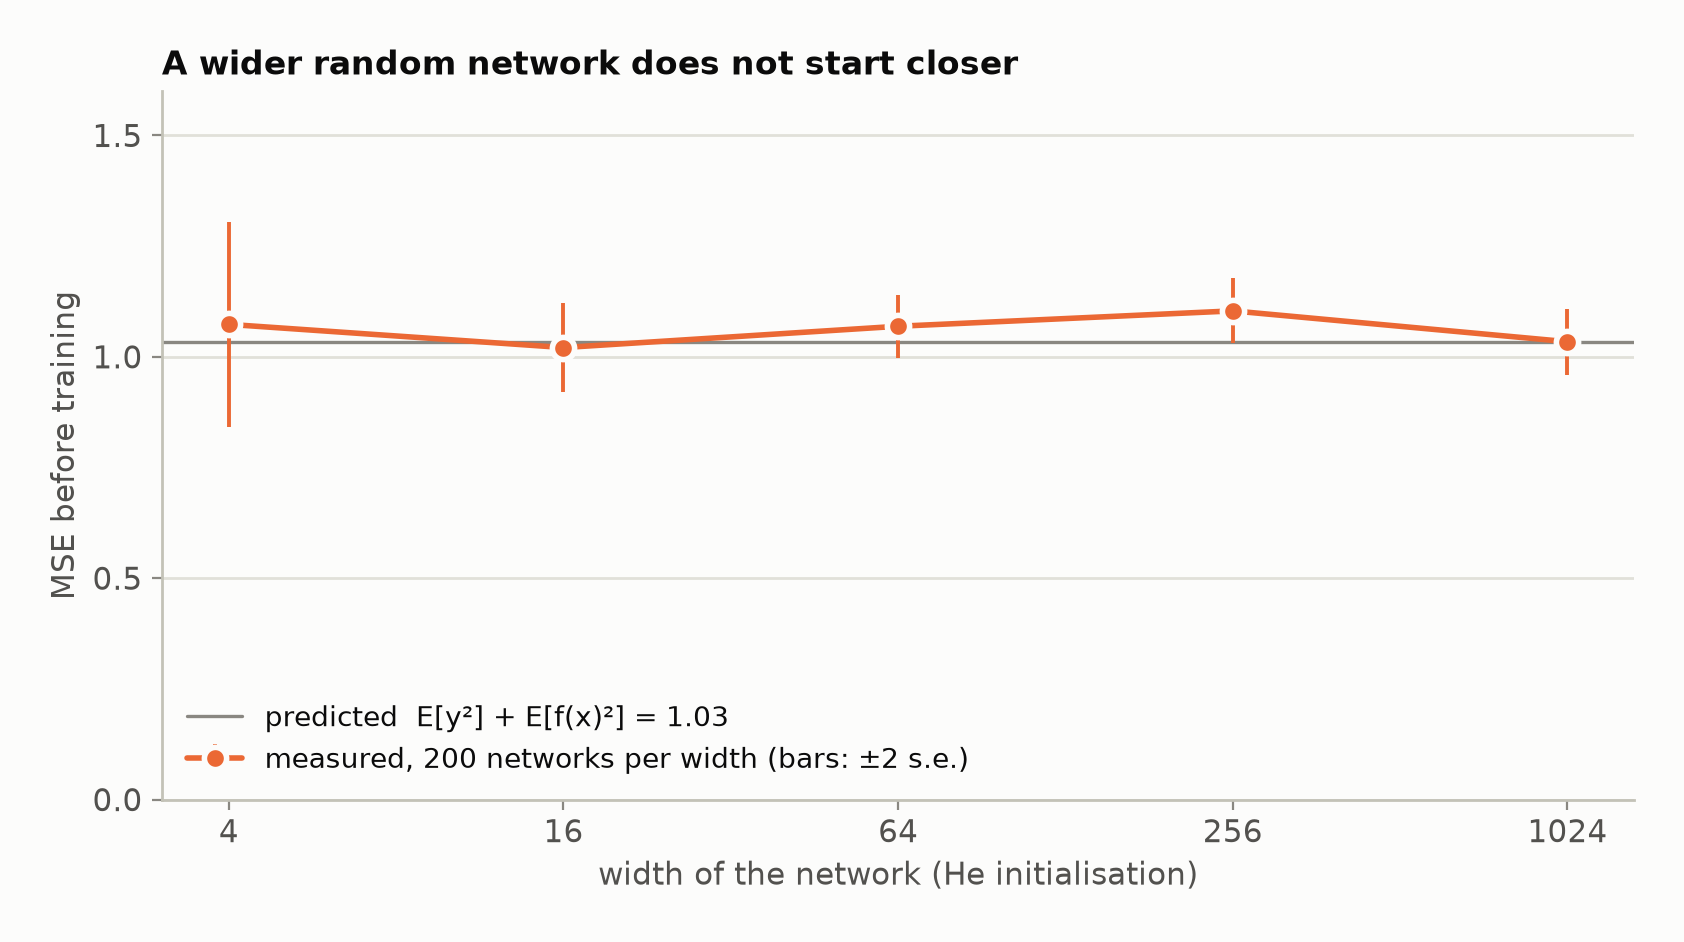
\includegraphics[width=0.74\linewidth]{../graphs/readme_initial_mse.png}
  \caption{Initial squared error of random ReLU networks under He
  initialisation (\cref{tab:mse}), with the prediction of \cref{cor:he}. Bars
  are $\pm2$ standard errors.}
  \label{fig:mse}
\end{figure}

\begin{table}[h]
  \caption{Random ReLU networks with a one-dimensional input: all sizes
  ($\pm$ one standard error over 300 networks; no training). Setup and caveats
  as in \cref{sec:nets}. Reference curves measured by the same code: the
  diagonal $y=x$ has length $2.83$ and distance $0.520$; a sine with one period
  across the box, $4.61$ and $0.351$; a sine with 16 periods, $64.07$ and
  $0.021$.}
  \label{tab:relu-full}
  \centering
  \begin{tabular}{rrrccc}
    \toprule
    width & hidden layers & parameters & arc length & turns & nearest-point \\
    \midrule
      2 & 2 &      12 & $3.446\pm0.040$ &  0.47 & $0.4808\pm0.0052$ \\
      4 & 2 &      32 & $3.571\pm0.037$ &  1.47 & $0.4540\pm0.0050$ \\
      8 & 2 &      96 & $3.512\pm0.034$ &  2.42 & $0.4398\pm0.0049$ \\
     16 & 2 &     320 & $3.604\pm0.035$ &  3.16 & $0.4231\pm0.0046$ \\
     32 & 2 &    1152 & $3.571\pm0.034$ &  4.39 & $0.4269\pm0.0046$ \\
     64 & 2 &    4352 & $3.559\pm0.035$ &  5.89 & $0.4269\pm0.0045$ \\
    128 & 2 &   16896 & $3.636\pm0.037$ &  8.18 & $0.4179\pm0.0046$ \\
    256 & 2 &   66560 & $3.577\pm0.036$ & 11.54 & $0.4286\pm0.0047$ \\
    512 & 2 &  264192 & $3.599\pm0.034$ & 15.11 & $0.4257\pm0.0046$ \\
    \midrule
     64 &  1 &    192 & $3.417\pm0.034$ &  3.05 & $0.4428\pm0.0047$ \\
     64 &  2 &   4352 & $3.613\pm0.037$ &  5.90 & $0.4256\pm0.0047$ \\
     64 &  3 &   8512 & $3.761\pm0.037$ &  8.39 & $0.4116\pm0.0048$ \\
     64 &  4 &  12672 & $3.900\pm0.039$ & 10.85 & $0.3938\pm0.0044$ \\
     64 &  6 &  20992 & $4.058\pm0.043$ & 15.67 & $0.3882\pm0.0044$ \\
     64 &  8 &  29312 & $4.368\pm0.049$ & 20.80 & $0.3643\pm0.0042$ \\
     64 & 12 &  45952 & $4.865\pm0.062$ & 28.88 & $0.3431\pm0.0040$ \\
     64 & 16 &  62592 & $5.100\pm0.075$ & 36.46 & $0.3433\pm0.0046$ \\
    \bottomrule
  \end{tabular}
\end{table}

\section{Lean names}
\label[appendix]{app:lean}

\begingroup\raggedright
The Lean project is in the folder \texttt{lean/} of the repository, built with
Lean 4.36.0-rc1 and the Mathlib commit recorded in
\texttt{lean/lake-manifest.json}. Each file is \texttt{lean/SquigglyLine/<name>.lean}.

\begin{itemize}\setlength{\itemsep}{1pt}
\item \cref{thm:sandwich}: \texttt{Sandwich}, \lean{nearestDist\_le\_verticalDist},
\lean{verticalDist\_le\_of\_lipschitz}.
\item \cref{thm:marginal} and \cref{cor:phase}: \texttt{Marginal},
\lean{expected\_residualLoss\_congr}; \texttt{RandomPhase},
\lean{marginal\_randomPhaseWave\_eq}; \texttt{Verdict},
\lean{not\_learningClaim\_sineWave}.
\item \cref{thm:tube}: \texttt{Coverage},
\lean{integral\_infDist\_eq\_integral\_uncovered}.
\item \cref{thm:cover}: \texttt{Oscillation},
\lean{nearestDist\_le\_of\_coversWithin},
\lean{verticalDist\_le\_of\_lipschitz\_of\_coversWithin},
\lean{expected\_nearestDist\_le}.
\item \cref{thm:sine}: \texttt{SineCloser},
\lean{sineWave\_nearestDist\_bounds},
\lean{tendsto\_expected\_nearestDist\_sineWave}; collected in
\texttt{SquigglyLineTheorem}, \lean{squiggly\_line\_theorem}.
\item \cref{prop:path,prop:more}: \texttt{LinearModel}, \lean{residual\_along},
\lean{exists\_within\_budget}, \lean{travel\_coprod\_le}.
\item \cref{thm:kernel}: \texttt{Kernel}, \lean{residual\_gradientStep},
\lean{travel\_eq\_norm\_of\_kernelInverse}, \lean{travel\_eq\_of\_kernel\_eq},
\lean{residual\_iterate\_gradientStep\_eq}.
\item \cref{cor:rate}: \texttt{ExchangeRate}, \lean{TightFeatures.travel\_eq};
\texttt{MarkovChains}, \lean{TightFeatures.residual\_iterate\_gradientStep},
\lean{TightFeatures.residual\_gradientStep\_inv}.
\item \cref{app:chains}: \texttt{NarrowChain}, \lean{narrowChain\_neverTurns};
\texttt{Depth}, \lean{iterate\_tent\_dyadic}; \texttt{Bridge},
\lean{sin\_sq\_iterate\_tent}; \texttt{Polarizer}, \lean{relu2\_nearest},
\lean{fan\_of\_le\_pi\_div\_two}, \lean{fan\_of\_pi\_div\_two\_le},
\lean{iterate\_fan}; \texttt{ThreePolarizers}, \lean{malus},
\lean{throughPlates\_light}, \lean{three\_polarizers},
\lean{quarter\_turn\_arrives}; \texttt{MarkovChains},
\lean{merged\_stays\_merged}, \lean{card\_image\_runLayers\_append\_le},
\lean{dead\_stays\_dead}.
\end{itemize}
\endgroup
